% Created 2023-04-24 Mon 23:54
% Intended LaTeX compiler: pdflatex
\documentclass[12pt]{article}

%%%% settings when exporting code %%%% 

\usepackage{listings}
\lstdefinestyle{code-small}{
backgroundcolor=\color{white}, % background color for the code block
basicstyle=\ttfamily\small, % font used to display the code
commentstyle=\color[rgb]{0.5,0,0.5}, % color used to display comments in the code
keywordstyle=\color{black}, % color used to highlight certain words in the code
numberstyle=\ttfamily\tiny\color{gray}, % color used to display the line numbers
rulecolor=\color{black}, % color of the frame
stringstyle=\color[rgb]{0,.5,0},  % color used to display strings in the code
breakatwhitespace=false, % sets if automatic breaks should only happen at whitespace
breaklines=true, % sets automatic line breaking
columns=fullflexible,
frame=single, % adds a frame around the code (non,leftline,topline,bottomline,lines,single,shadowbox)
keepspaces=true, % % keeps spaces in text, useful for keeping indentation of code
literate={~}{$\sim$}{1}, % symbol properly display via latex
numbers=none, % where to put the line-numbers; possible values are (none, left, right)
numbersep=10pt, % how far the line-numbers are from the code
showspaces=false,
showstringspaces=false,
stepnumber=1, % the step between two line-numbers. If it's 1, each line will be numbered
tabsize=1,
xleftmargin=0cm,
emph={anova,apply,class,coef,colnames,colNames,colSums,dim,dcast,for,ggplot,head,if,ifelse,is.na,lapply,list.files,library,logLik,melt,plot,require,rowSums,sapply,setcolorder,setkey,str,summary,tapply},
aboveskip = \medskipamount, % define the space above displayed listings.
belowskip = \medskipamount, % define the space above displayed listings.
lineskip = 0pt} % specifies additional space between lines in listings
\lstset{style=code-small}
%%%% packages %%%%%

\usepackage[utf8]{inputenc}
\usepackage[T1]{fontenc}
\usepackage{lmodern}
\usepackage{textcomp}
\usepackage{color}
\usepackage{graphicx}
\usepackage{grffile}
\usepackage{wrapfig}
\usepackage{rotating}
\usepackage{longtable}
\usepackage{multirow}
\usepackage{multicol}
\usepackage{changes}
\usepackage{pdflscape}
\usepackage{geometry}
\usepackage[normalem]{ulem}
\usepackage{amssymb}
\usepackage{amsmath}
\usepackage{amsfonts}
\usepackage{dsfont}
\usepackage{array}
\usepackage{ifthen}
\usepackage{hyperref}
\usepackage{natbib}
%
%%%% specifications %%%%
%
\usepackage{ifthen}
\usepackage{xifthen}
\usepackage{xargs}
\usepackage{xspace}
\newcommand{\first}{1\textsuperscript{st} }
\newcommand{\second}{2\textsuperscript{nd} }
\newcommand{\third}{3\textsuperscript{rd} }
\newcommand{\myname}[1]{Ozenne, B.}
\RequirePackage{fancyvrb}
\DefineVerbatimEnvironment{verbatim}{Verbatim}{fontsize=\small,formatcom = {\color[rgb]{0.5,0,0}}}
\RequirePackage{titlesec} % rename sections
\RequirePackage{colortbl} % arrayrulecolor to mix colors
\RequirePackage{setspace} % to modify the space between lines - incompatible with footnote in beamer
\renewcommand{\baselinestretch}{1.1}
\geometry{top=1cm}
\RequirePackage{colortbl} % arrayrulecolor to mix colors
\RequirePackage{pifont}
\RequirePackage{relsize}
\newcommand{\Cross}{{\raisebox{-0.5ex}%
{\relsize{1.5}\ding{56}}}\hspace{1pt} }
\newcommand{\Valid}{{\raisebox{-0.5ex}%
{\relsize{1.5}\ding{52}}}\hspace{1pt} }
\newcommand{\CrossR}{ \textcolor{red}{\Cross} }
\newcommand{\ValidV}{ \textcolor{green}{\Valid} }
\usepackage{stackengine}
\usepackage{scalerel}
\newcommand\Warning[1][3ex]{%
\renewcommand\stacktype{L}%
\scaleto{\stackon[1.3pt]{\color{red}$\triangle$}{\tiny\bfseries !}}{#1}%
\xspace
}
\hypersetup{
citecolor=[rgb]{0,0.5,0},
urlcolor=[rgb]{0,0,0.5},
linkcolor=[rgb]{0,0,0.5},
}
\RequirePackage{epstopdf} % to be able to convert .eps to .pdf image files
\RequirePackage{capt-of} %
\RequirePackage{caption} % newlines in graphics
\RequirePackage{pdfpages} % newlines in graphics
\usepackage[most]{tcolorbox}
\RequirePackage{enumitem} % to be able to convert .eps to .pdf image files
\definecolor{light}{rgb}{1, 1, 0.9}
\definecolor{lightred}{rgb}{1.0, 0.7, 0.7}
\definecolor{lightblue}{rgb}{0.0, 0.8, 0.8}
\newcommand{\darkblue}{blue!80!black}
\newcommand{\darkgreen}{green!50!black}
\newcommand{\darkred}{red!50!black}
\usepackage{mdframed}
\definecolor{grayR}{HTML}{8A8990}
\definecolor{grayL}{HTML}{C4C7C9}
\definecolor{blueM}{HTML}{1F63B5}
\newcommand{\Rlogo}[1][0.07]{
\begin{tikzpicture}[scale=#1]
\shade [right color=grayR,left color=grayL,shading angle=60]
(-3.55,0.3) .. controls (-3.55,1.75)
and (-1.9,2.7) .. (0,2.7) .. controls (2.05,2.7)
and (3.5,1.6) .. (3.5,0.3) .. controls (3.5,-1.2)
and (1.55,-2) .. (0,-2) .. controls (-2.3,-2)
and (-3.55,-0.75) .. cycle;

\fill[white]
(-2.15,0.2) .. controls (-2.15,1.2)
and (-0.7,1.8) .. (0.5,1.8) .. controls (2.2,1.8)
and (3.1,1.2) .. (3.1,0.2) .. controls (3.1,-0.75)
and (2.4,-1.45) .. (0.5,-1.45) .. controls (-1.1,-1.45)
and (-2.15,-0.7) .. cycle;

\fill[blueM]
(1.75,1.25) -- (-0.65,1.25) -- (-0.65,-2.75) -- (0.55,-2.75) -- (0.55,-1.15) --
(0.95,-1.15)  .. controls (1.15,-1.15)
and (1.5,-1.9) .. (1.9,-2.75) -- (3.25,-2.75)  .. controls (2.2,-1)
and (2.5,-1.2) .. (1.8,-0.95) .. controls (2.6,-0.9)
and (2.85,-0.35) .. (2.85,0.2) .. controls (2.85,0.7)
and (2.5,1.2) .. cycle;

\fill[white]  (1.4,0.4) -- (0.55,0.4) -- (0.55,-0.3) -- (1.4,-0.3).. controls (1.75,-0.3)
and (1.75,0.4) .. cycle;

\end{tikzpicture}
}
\author{Brice Ozenne}
\date{}
\title{Teaching Portfolio}
\hypersetup{
 colorlinks=true,
 pdfauthor={Brice Ozenne},
 pdftitle={Teaching Portfolio},
 pdfkeywords={},
 pdfsubject={},
 pdfcreator={Emacs 26.3 (Org mode 9.4.6)},
 pdflang={English}
 }
\begin{document}

\maketitle

\section{Teaching responsabilities}
\label{sec:org3a5fd07}

\textbf{Current teaching activity} at the University of Copenhagen (KU) for
Phd students in medical sciences:
\begin{itemize}
\item \href{https://absalon.ku.dk/courses/47665}{Statistical analysis of repeated measurements}: \newline It is a 6
days, 5 ECTS, course taught in english with 40-50 students. Julie
Forman is the course director. \newline I am doing 3 lectures of 3
hours and 6 exercise classes of 3 hours. I have been doing the
practical in this course since 2015 and started to lecture two years
ago.
\item \href{https://absalon.ku.dk/courses/58764}{Epidemiological methods in medical research}: \newline It is a 10
days, 7 ECTS, course taught in english with 20-30 students. I am the
course director. \newline I am doing 3.5 lectures of 3 hours, 7
exercise classes of 3 hours, and 3 hours of oral assessment (student
presentation). I have run the course 3 times (since 2021).
\item \href{http://paulblanche.com/files/BasicStat2023.html}{Basic statistics}: \newline It is a 10 days, 8 ECTS, course taught in
english with 30 students. Paul Blanche is the course
director. \newline I am doing 1 lectures of 3 hours and 1 exercise
classe of 3 hours and 6 hours of oral assessment (student
presentation). I have taught in this course 2 times (since 2021).
\end{itemize}

\textbf{Past teaching activity}:
\begin{itemize}
\item in 2016 I have taught a 2 hours lecture to statistics students
(Master level) for the course \href{https://absalon.instructure.com/courses/2385}{Structural Equation Models} at KU.
\item between 2013 and 2015, I was a teaching assistant at the \href{https://mastersantepublique.univ-lyon1.fr/icap\_website/299/5382}{University
of Lyon 1} (France) for biostatistics students (Master level). I was
doing 18h of practical in a survival analysis course and 6 hours of
practical in a course about Bayesian statistics.
\end{itemize}

\newgeometry{top=3cm}

\section{Supervision}
\label{sec:orgd9f855a}

I am/have been an official supervisor or co-supervisor of:
\begin{itemize}
\item Tanne Ebert Jørgensen and Johanne Triantafyllou Lorenzen (Master
students in epidemiology, 2023) about the childcare and symptoms of
ADHD in the danish population. The main supervisor is Anne-Marie
Nybo Andersen from the section of epidemiology.
\item Simon Christoffer Ziersen (Ph.D in biostatistics, from 2021) about
target trial emulation in observational studies of epilepsy and
depression. The main supervisors are Esben Budtz-Jørgensen and
Thomas Alexander Gerds from the section of biostatistics.
\item Ramlah Sara Rehman (Bachelor in data science, 2021) about clustering
trajectories of the cortisol concentration, comparing several
clustering algorithms. This was a co-supervision with Melanie
Ganz-Benjaminsen from the department of computer science.
\item Alice Brouquet-Laglaire (Master 2 in biostatistics, 2019) about the
comparison of inference methods for generalized pairwise
comparisons. The main supervisor was Julien Péron from the
University Lyon 1 (France).
\item Ceren Tozlu (Master 2 in biostatistics, 2014) about comparison of
classification methods for tissue outcome after ischemic stroke. The
main supervisor was Delphine Maucort-Boulch from the University Lyon
1 (France) This master project has lead to a publication
\citep{tozlu2019comparison}
\end{itemize}

\bigskip

I am also a statistical consultant at the Neurobiology research unit
(NRU). I help medical doctors, psychologists, neuro-scientists,
biologists, engineer of various levels (mainly Master and
Ph.D. students) to plan and perform data analysis. My Tuesday
afternoon is dedicated to this activity: understanding the context and
research question(s), advising and explain statistic concepts and
methods. \newline Via these consultations, I have informally
supervised many Master and Ph.D. students. For instance Kristin
Köhler-Forsberg (medical Ph.D., from 2016 until 2020) who I helped to
use latent variable models to anlayse PET data
\citep{kohler2023serotonin,kohler2022concurrent}, Camilla Borgsted
(Ph.D. in neuroscience from 2018 until 2022) who I helped to use
linear mixed model to analyse fMRI data \citep{borgsted2018amygdala}, or
Søren Vinther Larsen (medical Ph.D., from 2020) who I helped with
mulitple comparison adjustment, handling of detection limit, survival
analysis and study design \citep{larsen2020oral,larsen2022impact}.


\section{Pedagogical development projects}
\label{sec:orgc8baf40}

\textbf{LMMstar}: a common student feedback about practicals of the course
"Statistical analysis of repeated measurements" was the difficulty to
work with repeated measurements in \Rlogo. Student felts it required
substantial programming expertise and data management was very time
consuming and were sometimes discuraged. It is true that the code was
sometimes complex, relying on different software packages. Software
limitations also meant that ideas developped during the lecture could
not be examplified in the practicals. \newline During the last three
years I have developped, in collaboration with Julie Forman, a
software facilating student interactions with repeated measurements,
and in particular the use of linear mixed models. Having a dedicated
software solution to compute relevant summary statistics (mean,
correlation, number of missing data) and fit statistical models with
default option suited to the course has greatly facilitated the
programming aspect (see appendix \ref{appendix-software} for two examples),
freeing some time to discuss modeling and interpretation. Removing the
feasibility issue also leads to a better alignement between what is
being taught during the lectures and what is being done during the
exercises. \newline This is still an on-going project since models for
binary and count data are not yet included in the software. We would
also like to write pedagogical material about the analysis of repeated
measurements targeted to our students and applied researchers.

\bigskip

\textbf{Mini Epi seminar}: when I took over the epidemiology course there was
no student assessment (other than attendance). I believe that having
some formative assessment is useful to the student to get feedback on
knowledge, skills, or competences that has been acquired. Instead of
an exam I favor a form authentic assessment where students are asked
to present one of their research project in relation to concepts seens
during the course. The audience (other students and the teacher) then
engage in a conversation with the student about working assumptions,
limitations, and perspectives. Students usually really like this
activity as it links the content of the course to their
research. \newline To engage ealry the students and ensure that the
activity is well understood, I recently introduced a peer-feedback
session mid-way through the course. Students send me the output of
this peer-feedback session on which I give feedback. See appendix
\ref{appendix-seminar} for details and discussion about this
activity. \newline The quality and learning achieved during session
depends on the students. A very large majority of them take it
seriously, delivering interesting presentations and asking
questions. This year was especially successful, maybe partly thanks to
the introduction of the peer-feedback session.


\clearpage


\section{Formal pedagogical training}
\label{sec:org9891d48}

I have taken two courses about pedagogy: the \href{https://absalon.ku.dk/courses/58829}{Introduction to
University Pedagogy} in April 2022 and recently finished \footnote{for the
practical part I am missing the observations with the educational
supervisor. They are planned May 15th.} the theoretical part of the
\href{https://absalon.ku.dk/courses/58114}{University Pedagogy} (Universitetspædagogikum). My pedagogical project
was about implementing a peer feedback session that is described and
evaluated in appendix \ref{appendix-seminar}.

\section{Pedagogical approach}
\label{sec:orgb8a3d5d}

Teaching is for me sharing my entousiasm and my knowledge about a
subject, hoping to stimulate the appropriation of statistical concepts
and the curiosity of the students.

\bigskip

While I try to examplify and illustrate statistical concepts (e.g see
appendix \ref{appendix-illustration}), I strongly believe that proper
understanding of biostatistics concepts require some mathematical
representation. The level of formalism used when teaching will
dependent on the audience (medical vs. mathematic students) and on the
targeted level of understanding. This being said, mathematics are here
to explicit an idea, not to obscure it. So I also believe that
learning biostatistics involve developping its intuition, for instance
to understand the practical implications of a statistical hypothesis
(e.g. see appendix \ref{appendix-intuition}). Being lucid and explicit
about hypotheses withstanding a scientific investigation is
suprisingly difficult to master but a key part of biostatistics.

\bigskip

After several years of teaching, I have come to realize that a clear,
rigorous but intuitve explaination of statistical concepts requires
quite a substancial expertise on the topic. Examples or experience
from research project are generally approciated by students. I
therefore try, when possible and relevant, to relate my teaching
activity to my research activity. The LMMstar package is an example of
interconnexion between the two, initially motivated by the teaching
but made possible by knowledge acquired during research projects.

\bigskip

Finally I try to develop a learning environment open to discussion and
where the students feel confortable. Having interactions with students
during lectures and practicals to assess their understanding is not
only critical to adjust my teaching but also motivating. Using humor,
being supportive, taking the time to discuss with the students, and
showing vulnerability (e.g. mentionning mistakes I have made in the
past) seems to help having this safe learning environment.




\section{Personal development as a teacher}
\label{sec:orgb0f6deb}

The formal training I received during the University Pedagogy course
made me question my pedagogical approach and experience different
teaching technics, often based on group work and use of online-tools
(polls \& quizzes):
\begin{itemize}
\item it helped me better structure my teaching around intended learning
objectives (ILOs). I have realized that \textbf{each ILOs should be tested
during the lecture with short exercises} (see appendix
\ref{appendix-quizz} for an example). These short exercises provide
feedback to the students and the teacher about whether the knowledge
or skill has been acquired. It also creates variations during the
lecture which is beneficial to the student attention.

\item it made me reflect about the role of the teacher and the student in
the learning process. The student has the central role whereas the
teacher is here to facilitate the interaction between the student
and a subject. Indeed most students learn by doing and by
appropriation. I am in a process to \textbf{reduce the curriculum seen
during lecture or practicals and rely self study} for technical
skills. This leave more time during the class for experimentation
and discussion. The self study is supported by the lecture notes,
exercise solutions, or scientific articles. \newline
As an example, I have greatly reduced the attention given to
programming in the Epidemiology course (e.g. the code and software
output are given in most of the exercices). Learning programming is
left to self study even though I happily answer any question and
have a dedicated section in each of my lecture notes.

\item it provided me tools to \textbf{create a safe learning environment}. For
instance when a student answer a question, I would (try to) not
immediatly qualify it (correct or incorrect answer). Instead ask the
opinion of other students or ask a follow-up question to make the
student reflect/orient them in the right direction.

\item it stressed the importance of \textbf{engaging the student} using an
inductive approach, e.g. based on a motivating example where there
is a need for statistical tools. I generally use classical
statistical paradoxes (see appendix \ref{appendix-paradox} for an
example), as find a simple but realistic example for a specific ILO
is challenging - often realistic examples are complex and would cover
several ILOs.
\end{itemize}

Discussions and teaching material from colleagues have been a great
source of inspiration. They have also contributed to my evolution as a
teacher but in a more subtle and continuous way that will not explicit
here.

\section{References}
\label{sec:org842ef63}
\begingroup
\renewcommand{\section}[2]{}
\bibliographystyle{apalike}
\bibliography{publicationBO}

\endgroup

\appendix
\titleformat{\section}
{\normalfont\Large\bfseries}{Appendix~\thesection}{1em}{}

\clearpage

\section{Old vs. new software solution}
\label{appendix-software}
\subsection{Computing summary statistics}
\label{sec:orgee1af05}

\RecustomVerbatimEnvironment{verbatim}{Verbatim}{formatcom = {\color[rgb]{0.5,0,0}}}

Initially, we were teaching the students to use the \texttt{aggregate}
function to evaluate the mean and other statistics per timepoint:
\lstset{language=r,label= ,caption= ,captionpos=b,numbers=none}
\begin{lstlisting}
w.summaries <- aggregate(glucagonAUC~time, data=gastricbypassL,
                         FUN = function(iAUC){
  c("observed" = sum(!is.na(iAUC)),
    "missing" = sum(is.na(iAUC)),
    "mean" = mean(iAUC, na.rm = TRUE),
    "sd" = sd(iAUC, na.rm = TRUE),
    "min" = min(iAUC, na.rm = TRUE),
    "median" = median(iAUC, na.rm = TRUE),
    "max" = max(iAUC, na.rm = TRUE))},
  na.action=na.pass)
                               
w.summaries <- data.frame(w.summaries[1],w.summaries[[2]])
print(w.summaries, digits=4)

\end{lstlisting}

\begin{verbatim}
           time observed missing  mean   sd  min median   max
1 3monthsBefore       20       0  7860 3781 2500   6786 16798
2   1weekBefore       19       1  7149 3289 2376   6202 16300
3    1weekAfter       19       1 16954 6153 7906  16269 29980
4  3monthsAfter       20       0 11063 4479 4551  10911 23246
\end{verbatim}


While this is a very flexible approach, it was difficult for medical
students to understand. Instead we now use the \texttt{summarize} function
from LMMstar which has well suited default output for the applications
we have in mind in the course:
\lstset{language=r,label= ,caption= ,captionpos=b,numbers=none}
\begin{lstlisting}
summarize(glucagonAUC ~ time|id, data = gastricbypassL, na.rm = TRUE)
\end{lstlisting}

\begin{verbatim}
           time observed missing      mean       sd    min        q1  median       q3      max
1 3monthsBefore       20       0  7860.443 3781.459 2500.5  5185.875  6786.0 10337.51 16797.75
2   1weekBefore       19       1  7148.589 3288.933 2376.0  5113.500  6202.5  8082.75 16300.50
3    1weekAfter       19       1 16953.671 6152.867 7906.5 12466.500 16269.0 20271.00 29979.75
4  3monthsAfter       20       0 11063.025 4479.478 4551.0  7914.225 10911.0 12340.50 23245.50

 Pearson's correlation: 
              3monthsBefore 1weekBefore  1weekAfter 3monthsAfter
3monthsBefore     1.0000000  0.83158346  0.13902263   -0.2496747
1weekBefore       0.8315835  1.00000000 -0.09418889   -0.2232003
1weekAfter        0.1390226 -0.09418889  1.00000000    0.5988570
3monthsAfter     -0.2496747 -0.22320033  0.59885696    1.0000000
\end{verbatim}

Note that key arguments, such as how to handle missing data are kept
to stress their importance to the students. One functionality has been
added to obtain the correlation matrix by explaining in the formula
interface how the data are grouped. This enable to have a single
statement outputing all the standard descriptive statistics. The
student can now focus on the interpretation of these statistics and
their implication in term of statistical modeling.

\subsection{Fitting linear mixed models}
\label{sec:org225c4a8}

Another difficulty was to estimate linear mixed models with
unstructured covariance patterns. We advocate their use during the
course but, at the time, the \Rlogo syntax was complicated:
\lstset{language=r,label= ,caption= ,captionpos=b,numbers=none}
\begin{lstlisting}
fit.main <- gls(glucagonAUC ~ time,
                data = gastricbypassL,
                correlation = corSymm(form=~as.numeric(time)|id),
                weights = varIdent(form=~1|time),
                na.action=  na.exclude,
                control = glsControl(opt="optim"))
logLik(fit.main)
\end{lstlisting}

\begin{verbatim}
'log Lik.' -712.161 (df=14)
\end{verbatim}


We developped our own mixed model implementation, with a simpler
syntax that stresses the choice of the covariance structure (one of
the learning point of the course):
\lstset{language=r,label= ,caption= ,captionpos=b,numbers=none}
\begin{lstlisting}
fit.main2 <- lmm(glucagonAUC ~ time,
                data = gastricbypassL,
                repetition = ~time|id,
                structure = "UN")
logLik(fit.main2)
\end{lstlisting}

\begin{verbatim}
[1] -712.161
\end{verbatim}


\clearpage 

\section{Pedagogy project (without appendix)}
\label{appendix-seminar}

\vspace{-1cm}

\begin{figure}[!h]
\centering
\tcbox[colback=blue!5,boxsep=5mm,boxrule=1mm]{
\includegraphics[page=1, scale=.75, clip, trim=20mm 27mm 20mm 5mm]{figures/finalProject.pdf}}
\end{figure}

\clearpage

\foreach \mypage in {2,...,5}{

\begin{figure}[!h]
\centering
\tcbox[colback=blue!5,boxsep=5mm,boxrule=1mm]{
\includegraphics[page=\mypage, scale=.75, clip, trim=20mm 27mm 20mm 5mm]{figures/finalProject.pdf}}
\end{figure}

}
% 
\includepdf[pages=-,clip, trim=20mm 27mm 20mm 5mm,
%     pages=-,
%     frame,
%     scale=.7,
%     pagecommand={}]{figures/finalProject.pdf}

\section{Example of teaching material}
\label{sec:orga69eb23}

\subsection{Course on Epidemiology (illustration)}
\label{appendix-illustration}
Slide explaining how to evaluate the risk of a disease based on the
incidence rate. The intuition behind the mathematical formula is
illustrated via a series of graphs.

\begin{figure}[!h]
\centering

\includegraphics[trim={0 0 0 0}, page = 6, width=1\textwidth]{./figures/L5-confounding.pdf}
\label{fig:lmm-slide-wiw}
\end{figure}

\clearpage

\subsection{Course on Epidemiology (intuition)}
\label{appendix-intuition}
Slide illustrating the implications of the independent censoring
assumption used by the Kaplan Meier estimator. This estimator can be
re-formulated as a simple weighted average, where the weight accounts
for the lost to follow-up, and help expliciting implications of the
Kaplan Meier approach.

\begin{figure}[!h]
\centering
\includegraphics[trim={0 0 0 0}, page = 24, width=1\textwidth]{./figures/L13-registry.pdf}
\label{fig:lmm-slide-wiw}
\end{figure}

\clearpage

\subsection{Course on repeated measurement (exercise)}
\label{appendix-quizz}
Exercise slide where the students are asked to associate a study
design (symbolized by a graph) with a correlation structure. This
tests the ILO: "Describing a correlation structure via a graph"
\begin{figure}[!h]
\centering
\includegraphics[trim={0 0 0 0}, page = 21, width=1\textwidth]{./figures/repMes-randomEffects-lecture.pdf}
\label{fig:lmm-slide-wiw}
\end{figure}

\clearpage

\subsection{Course on Epidemiology (paradox)}
\label{appendix-paradox}
Example of statistical paradox that should make the student reflect
upon:
\begin{itemize}
\item what do we actually mean by \emph{beneficial} or \emph{having an effect}?
\item when one should or should not adjust an analysis for covariates?
\end{itemize}

\begin{figure}[!h]
\centering

\includegraphics[trim={0 0 0 0}, page = 20, width=1\textwidth]{./figures/L5-confounding.pdf}
\label{fig:lmm-slide-wiw}
\end{figure}

After a short reflection time, I will ask the opinion of the
students. I will not provide the answer but stress that paradoxes
challenge our intuition and a more objective approach, counterfactuals
and directed acyclic graphs (DAGs), are needed to resolve the paradox
in a convicing way. When explaining counterfactuals and DAGs I would
relate them (as much as possible) to the paradox and the intuition of
the students.
\end{document}